% -*- TeX -*- -*- Soft -*-
%Daemon> filter=err+warn
%Daemon> custom_args="-synctex=1"
%Daemon> ini=pdflatex

\documentclass{article}
\usepackage{lscape}
\usepackage{amsmath, amsthm, amssymb}
\usepackage{a4wide}
\usepackage{gamesem}
\usepackage{pst-tree}
%\usepackage{xcolor}
\usepackage{pstring}
\usepackage{todonotes}
\usepackage{amsmath,amssymb,amsthm}
\usepackage{bcprules}

\theoremstyle{definition}
\newtheorem{definition}{Definition}[section]
\newtheorem{property}{Property}[section]
\newtheorem{proposition}{Proposition}[section]
\newtheorem{remark}{Remark}[section]
\newtheorem{theorem}{Theorem}[section]
\newtheorem{example}{Example}[section]
\newtheorem{observation}{Observation}[section]

\newcommand\Nodes{N}% set of nodes
\newcommand\NodesVar{N_{\sf var}}% set of nodes
\newcommand\NodesLmd{N_\lambda}% set of nodes

\newcommand{\ghostlmd}{{\lambda\!\!\lambda}}
\newcommand{\ghostvar}{\theta}

\newcommand{\affine}{{\sf aff}}
\newcommand{\normalizing}{{\sf norm}}
\newcommand{\branching}{{\sf branch}}

\newcommand{\travsetaffine}{{\travset^\affine}}
\newcommand{\travsetbr}{{\travset^\branching}}
\newcommand{\travsetnorm}{{\travset^\normalizing}}


\newcommand{\NodeHjByRoot}{\Nodes^{\filter\theroot}}

\newcommand{\rulefont}[1]{\mathbf{\sf #1}}
\newcommand{\enables}{\vdash}

\newcommand\pathset{{\mathcal{P}aths}}
\newcommand\arth{\textsf{arth}}

\author{William Blum}
\title{[Draft] Untyped Normalizing Traversals. \\
 {\small How to traverse and normalize untyped lambda terms via on-the-fly eta-expansion.}}

\begin{document}
\maketitle
\begin{abstract}
This note introduces a new method to traverse untyped lambda terms. It extends the notion of traversals introduced in my thesis \cite{BlumPhd} for the simply-typed lambda calculus (STLC) to the untyped lambda calculus (ULC), and yields a method to normalize terms.

Traversals were originally introduced by Ong to study higher-order recursion schemes used as generator of order-$0$ structures such as trees. In \cite{BlumPhd}, I extended the notion to the simply-typed lambda calculus by adding the (IVar) rule to account for free variables, and gave a concrete proof that traversals are isomoprhic to the game denotation of a simply-typed term through the `core projection' operation.

The adapation to the untyped setting adds several new ingredients:
(i) The (Lam) and (Var) rules are augmented to implement eta-expansion when there is an insufficient number of variable names in the lambda node of a redex to be able to traverse it.
(ii) The eta-expansion is performed `on-the-fly`, as needed, at every point where the traditional STLC traversal would normally get stuck.
(iii) The concept of ``ghost'' nodes is introduced to model imaginary nodes in the computation tree that progressively appear as eta-expansions are performed on the subterms.
(iv) The computation tree itself does not get modified during eta-expansion. Ghost nodes are only added to the traversal and are only ``visible'' in the context where they get introduced.
(v) The (IVar) rule, introduced in my thesis to model free variables, is constrained by a quantity called the `arity threshold` which can be calculated in linear time from the traversal itself. This limits the non-deterministic branching factor of this rule, which is required to guarantee that the normalization procedure terminates when the beta-normal form exists.

I've implemented the normalization algorithm in the HOG tool. I provide some examples of normalized terms in the last section.

{\bf TODO:}

(i) Adapt the proof of the game semantics correspondence theorem from my thesis to this setting, perhaps using Andrew Ker's game model of ULC.

(ii) Establish connection with previous work by Daniil Berezun and Neil Jones on traversals compilation for ULC.
\end{abstract}

\section{Background}

In \cite{BlumPhd} we establish the correspondence between the theory of traversals and Game semantics for the simply-typed lambda calculus (STLC). The proof in the thesis relies on several ingredients:
\begin{enumerate}
  \item The introduction of a new traversal rule \rulenamet{IVar} to model free variables;
  \item A formal definition of the notion of \defname{interaction game semantics} corresponding to the game denotation of a term in the usual sense but where internal moves are all revealed instead of hidden;
  \item The definition of various operations on traversals, in particular the notion of \defname{traversal core} which preserves only the ``essence'' of a traversal.
\end{enumerate}


One can then show that, for every simply-typed term $\Gamma \entail M :T$,
there is a bijection $\varphi_M$ from the set of traversals of $M$ to the revealed interaction game denotation of $M$, further there is a bijection between the standard game denotation of $M$ and its standard innocent game denotation. Formally:
\begin{theorem}[STLC Game Semantics and Traversals (Theorem 4.96 in \cite{BlumPhd}]
\label{thm:correspondence}
For every simply-typed term $\Gamma \entail M :T$ there exists two bijections
$\phi_M$ and $\psi_M$:

\begin{eqnarray*}
 \varphi_M  &:& \travset(\Gamma \entail M : T)^\star \stackrel{\cong}{\longrightarrow} \syntrevsem{\Gamma \entail M :T} \\
 \psi_M  &:& \travset(\Gamma \entail M : T)^{\filter \theroot} \stackrel{\cong}{\longrightarrow} \sem{\Gamma \entail M :T} \enspace .
\end{eqnarray*}

where $\syntrevsem{\Gamma \entail M : T}$ denotes the interaction game denotation of $M$, $\sem{\Gamma \entail M : T}$ denotes the innocent game denotation of $M$,
$\travset(M)^\star$ denotes the set of traversals where application nodes are removed, and $\travset(M)^{\filter
\theroot}$ denotes the set of traversal cores of $M$ (\ie traversal projected to the root of the tree).
\end{theorem}

\subsection{Normalizing terms with traversals}

The \defname{projection with respect to the root} of a traversal $t$, noted $t\filter {\theroot}$, gives what we call the \defname{core} of the traversal consisting of the subsequence of nodes that are hereditarily justified by the root. By the correspondence theorem the traversal cores are precisely plays from the game denotation of the term.
Because the traversals P-views (noted $\pview{t}$ for every traversal $t$) correspond to paths in the tree representation of the term (\cite{BlumPhd}, Proposition 4.29), this yields a method to calculate the beta-normal form of any STLC term $M$:
\begin{enumerate}
  \item Enumerate traversals of $M$;
  \item For each traversal $t$, calculate its traversal core $t \filter \theroot$. This gives a play in $\sem{M}$;
  \item Calculate the P-view of the traversal core: $\pview{t\filter \theroot}$;
  \item Apply the Correspondence bijection to get the corresponding path in the tree representation of the $\beta$-nf of $M$.
\end{enumerate}


\begin{remark}
All the traversal rules are deterministic except \rulenamet{IVar}. The rule \rulenamet{IVar} gives two non-deterministic choices: (i) the variable to pick in the O-view,
(ii) the child lambda node to pick amongst the picked variable's children.
A consequence of this definition is that even for terms having a normal form (and in particular even for beta-normal terms), the set of traversals can be infinite, and traversals can be infinitely long.
E.g. Take the term $\lambda f . f (\lambda x. x)$. We have that $\lambda f \cdot f \cdot (\lambda x \cdot  x)^k$ is a traversal for all $k\geq0$. Viewed from a game semantic perspective, those traversals accounts for all the possible denotations of the function parameter $f$: observe that for each $k$, there exists a term that applies its argument $k$ times: $\lambda y . y (y ( \ldots y)) $.

\todo{Type my handwritten notes with proof explaining this in more details.}
For the sake of computing the beta-normal form of a term, however, it's only necessary to traverse finitely many finite traversals (provided that the normal form exists). Effectively, this means limiting the rule \rulenamet{IVar} so that it traverse only nodes leading to paths in the computation tree that are yet unexplored. In practice, it means that when choosing the next lambda node to visit, one can ignore nodes that are already present in the O-view.
\end{remark}

\textbf{Implementation}
This reduction method was implemented in the HOG tool mentioned in my thesis which lets you ``play the traversal game'' and calculate various types of projections including the one giving the traversal cores.

\todo{Cite Neil's paper and discussion.}
The question addressed in the present note is: can this method be extended to the untyped lambda calculus (ULC) following the same game-semantic argument but based on Ker's game model of the untyped lambda calculus instead of the game model of STLC?


\section{Definitions}

\subsection{Computation tree, enabling relation, justified sequences}

For an untyped lambda term $M$ we defined its \defname{computation tree} $\tau(M)$ the same way as for the STLC
except that we don't perform eta-long expansion. Consecutive lambda abstractions are still merged into a single nodes in the tree so as to maintain the alternation between lambda nodes (at odd level) and variable nodes (at even level).
Let $\Nodes$ be the set of nodes of the computation tree. We write $\NodesVar$ for the set of variable nodes, $\NodesLmd$ for lambda nodes, and $\Nodes_{@}$ for the application nodes.
We define the \defname{enabling relation} $\enables$ between nodes of the computation tree as the relation associating each lambda node to all the variable nodes that it binds, and every variable and application node to each of their child node. We write $m \enables_k \alpha$ to indicate that a lambda node $\alpha$ is the $k$th child of a variable or application node $m$ for some $k\geq0$; and $\alpha \enables_k m$ to indicate that the node $m$ is labelled by the $k$th variable bound by $\alpha$ for $k\geq1$. We write $\NodeHjByRoot$ to denotes the image of the root of the tree by the transitive closure of the enabling relation and we call it the set of nodes \defname{hereditarily enabled by the root}.

We call a \defname{justified sequence}, a sequences of nodes of $\Nodes$ where each node occurrence (except the very first one in the sequence) has an associated ``justification pointers'' or ``link'' pointing to a another node occurring before it in the sequence and respecting the enabling relation $\enables$. The target occurence of the link is called the ``justifier''.

We defined the \defname{arity} of a node as follows: the arity of a lambda node $\lambda x_1 \cdots x_k$ for $k\geq 0$ is denoted by $|\lambda x_1 \cdots x_k|$ and is defined as $k$; the arity of a variable node $x$, denoted $|x|$ is the number of children of $x$ in the computation tree; the arity of a $@$ node is the number of its children nodes minus 1.

\subsubsection{ULC ghost nodes}
For ULC, we extend the definition of nodes from STLC by introducing two infinite classes of ``imaginary'' nodes called \defname{ghost nodes}:
one class of ``ghost variable nodes'', denoted $\ghostvar$, and one class of ``ghost lambda nodes'', denoted $\ghostlmd$. By abuse of notation we will use $\ghostvar$ and $\ghostlmd$ to refer to particular elements of the two respective classes.

We will refer to nodes $\Nodes$ of the computation tree as \defname{structural nodes}, and nodes in $\ghostlmd$ and $\ghostvar$ as the \defname{ghost nodes}. We will write $\NodesLmd^\ghostlmd$ as a shortand for $\NodesLmd + \ghostlmd$
and $\NodesVar^\ghostvar$ as a shortand for $\NodesVar + \ghostvar$.

We extend the definition of the enabling relation $\enables$ to ghost nodes by induction as follows: for every (ghost) variable or application node $m$ and for all $k>|m|$ there is a ghost lambda node $\ghostlmd$ such that $m \enables_k \ghostlmd$; for all (ghost) lambda node $\alpha$ and all $k>|\alpha|$ there is a ghost variable node $\ghostlmd$ such that $\alpha \enables_k \ghostvar$.

Observe that every ghost variable and ghost lambda node is uniquely defined by its enabler node (possibly itself a ghost node) and the associated label $k\geq 1$.

Ghost nodes thus defined will be used as placeholders in \defname{justified sequences} to represent eta-expanded lambda nodes and variable nodes respectively.

By convention ghost variables and lambda nodes are given arity $0$.

\subsection{Traversals}

The set $\travset(M)$ of \defname{traversals} over an untyped lambda term $\tau(M)$ is a jsutified sequence of elements in $\Nodes + \ghostlmd + \ghostvar$ with associated pointers. It is defined by induction over the rules of Table \ref{tab:trav_rules}.

For any traversal $t$ we write $t^\omega$ to denote the last occurrence in traversal $t$, and $\jp(t)$ to denote the prefix of $t$ ending at the justifier of the last node of $t$.

We say that $t$ is an \defname{extension} of traversal $u$ if $u$ is a strict subsequence of $t$ sharing the same justification pointers.
A traversal that does not have any extension is a \defname{maximal traversal}.

We say that an occurrence of a node in a traversal is \defname{hereditarily justified by the root (occurrence)} if recursively following justification pointers starting from that occurrences leads to the initial occurrence of the root node in the traversal. An immediate property of traversal is that traversal occurrences that are hereditarily justified by the root correspond to nodes of the computation tree that are hereditarily enabled by the root: \ie they are all occurrences of nodes in $\NodeHjByRoot$.

Note that those rules closely match those of \cite{BlumPhd} for STLC. In the present setting of ULC, however, there are no interpreted constants therefore we don't need the rules \rulenamet{Value} and \rulenamet{InputValue} from the original presentation.

We now fix an untyped term and abbreviated its set of traversals as just $\travset$.

\begin{FramedTable}
\noindent {\bf Structural rules}
\begin{itemize}[]
\item\rulenamet{Root} The singleton sequence $r$ is in $\travset$ where $r$ is the root of the tree.
\end{itemize}

\begin{itemize}[]
    \item \rulenamet{Lam} If $t \cdot \alpha$ is a traversal where $\alpha\in\NodesLmd$ then so is
        $t \cdot \alpha \cdot n$ where $n$
        denotes $\alpha$'s unique child in $\tau(M)$ and its justifier is defined as follows. If $n$ is
        \begin{compactitem}
            \item an $@$-node then it has no justifier,
            \item in $\Nodes_{\sf fv}$ then it points
            to the only occurrence of the root in
            $\pview{t \cdot \alpha}$,
            \item in $\Nodes_{\sf var}\setminus \Nodes_{\sf fv}$ then it points to the only occurrence of its binder in
            $\pview{t\cdot \alpha}$.
        \end{compactitem}
    \item \rulenamet{Lam^\ghostlmd} If
  $\Pstr[0.5cm]{ t \cdot(alpha){\alpha} \cdot
(n){n} \cdot \ldots \cdot
(gl-n,40:i){\ghostlmd} \in\travset}$ for some prefix $t$, $\alpha \in \NodesLmd^\ghostlmd$ and $n \in\NodesVar^\ghostvar$ then
$$\Pstr[0.5cm]{ t \cdot(alpha){\alpha} \cdot
(n){n}
\cdot \ldots \cdot
(gl-n,40:i){\ghostlmd}\cdot (al-alpha,40:j){\ghostvar}
      \in\travset}$$
 where $j = |\alpha| + i - |n|$. (Intuition: the ghost placeholder $\ghostvar$ represents an occurrence of the $j$th variable that would be bound by lambda node $\alpha$ if the sub-term at node $\alpha$ were eta-expanded $i-|n|$ times.
 We have $i>|n|$ necessarily since the $i$th child of $n$ is a ghost variable node.)


    \item \rulenamet{App} If $t \cdot @$ is a traversal then so is \Pstr[0.4cm]{t \cdot (at) @  \cdot (a-at,40:0) \alpha} where $\alpha\in\NodesLmd$ is the $0$th child $\lambda$-node of $@$.
\end{itemize}

\emph{\bf Data - Input-variable rules}

If $t \cdot n$ is a traversal where $n \in \NodesVar^\ghostvar$ is hereditarily justified by the root:
\begin{itemize}[]
\item \rulenamet{IVar} If $n$ is a structural node then
for every node $m \in \NodesVar$ occurring in $\oview{t\cdot n}$
and every $k$th child $\alpha \in \Nodes_\lambda$ of $m$ (where $k\leq|m|$),
we have $t \cdot n \cdot \alpha \in \travset$ with $\alpha$ pointing to $m$ with label $k$.

\item \rulenamet{IVar^\eta} If $n$ is a ghost variable then
for every node $m\in \NodesVar$ occurring in $\oview{t\cdot n}$ and every $k>|m|$ we have $t \cdot n \cdot \ghostlmd \in\travset$, with $\ghostlmd$ pointing to $m$ with label $k$.
\end{itemize}

\emph{\bf Program - Copy-cat rules \underline{with on-the-fly eta-expansion}}

Suppose \Pstr[0.5cm]{t \cdot (n){n} \cdot (alpha){\alpha}
    \ldots (m-alpha,50:i){m} \in \travset} where $i>0$, $m \in \NodesVar^\ghostvar$ hereditarily justified by an $@$-node;
     $n \in \NodesVar^\ghostvar \union \Nodes_{@}$; and $\alpha \in \NodesLmd^\ghostlmd$. Then:

\begin{itemize}
  \item \rulenamet{Var} (No expansion) If $i \leq |n|$ then
  $$\Pstr[0.5cm]{ t  \cdot
(n){n} \cdot (lx){\alpha}  \ldots (x-lx,30:i){m}
    \cdot (letai-n,40:i){\lambda \overline{x}}
     \in\travset}$$
where $\lambda \overline{x} \in N$ is the $i$th child of $n$
(both structural nodes of the tree since $|n|\geq i>0$).

\item \rulenamet{Var^\eta} (Eta-Expansion) If $i > |n|$ then
  $$\Pstr[0.5cm]{ t \cdot
(n){n} \cdot (lx){\alpha}  \ldots (x-lx,30:i){m}
    \cdot (letai-n,40:i){\ghostlmd}
     \in\travset}$$
     where the ghost node $\ghostlmd$ represents the $i$th ghost child of $n$.
\end{itemize}

\caption{Traversal rules for the untyped lambda calculus (ULC).}
 \label{tab:trav_rules}
\end{FramedTable}

Ghost nodes appear in a traversal when the arity of a node is too low to continue a regular
structural traversal of the tree:
\begin{property}
If $\Pstr[0.5cm]{(x){x} \cdots (y-x,30:i){y}} \in \travset$ then
$$ y \in \ghostvar \mbox{ or } y \in\ghostlmd \iff i > |x|.$$

In particular for all $n\in\NodesVar$ and $\alpha\in\NodesLmd$:
\begin{enumerate}
\item $\Pstr[0.5cm]{(x){n} \cdots (y-x,30:i){\ghostlmd}} \in \travset \implies i > |n|$
\item $\Pstr[0.5cm]{(x){\alpha} \cdots (y-x,30:i){\ghostvar}} \in \travset \implies i > |n|$.
\end{enumerate}
\end{property}

\begin{remark}
The rule \rulenamet{Lam} is well defined. In particular it can be show as in STLC, that P-views are paths in the (possibly eta-expanded) tree thus $n$'s enabler occurs exactly once in the P-view.
\end{remark}

\begin{definition}
We call \defname{ghost materialization} instances of traversal rule application where the last occurrence in the traversal is
a ghost nodes, and the new node traversed, after applying some traversal rule, is a structural node.
\end{definition}

\begin{remark}[Only \rulenamet{Var} can materialize a ghost node]
Observet that among all the rules defined in Table \ref{tab:trav_rules}, the rule \rulenamet{Var} is the only rule that can materialize a structural node in $\Nodes$ from a traversal ending with a ghost node. This means that after traversing ghost nodes, the only way to come back to strucutural nodes is to visit a ghost variable node $\ghostvar$ with an application of rule \rulenamet{Var} of the following form:

$$\rulename{Var}\ \  \Pstr[0.5cm]{ t \cdot(beta){\beta} \cdot
(y){y} \cdot (l){\alpha}  \ldots (t-l,30:i){\ghostvar}
    \cdot (lx-y,40:i){\lambda \overline{x}}
     \in\travset}$$
where
\begin{itemize}
\item $y \in \NodesVar$
\item $\lambda \overline{x} \in \NodesLmd$ is the $i$th child lambda node of $y \in \NodesVar$,
\item $\alpha$ is either a structural lambda node in $\Nodes_\lambda$ or a ghost lambda node in $\ghostlmd$
\item $0\leq \alpha < i \leq |y|$.
\end{itemize}
\end{remark}




\section{Correspondence}
Following the STLC framework of my thesis, the rule \rulenamet{IVar} is defined so as to obtain the correspondence with game semantics: the nodes visited by this rule correspond to moves played by the Opponent in the game denotation. (We recall that in Game Semantics, the Opponent represents the environment of the program, or equivalently, the data passed to the program.
We aim to prove that this presentation yields an isomorphism between the set of traversals and the revealed game semantics of the ULC term, and subsequently that it yields an isomorphism between the standard game semantics and the set of traversal cores (i.e., projected wrt. the root):

\begin{theorem}[Correspondence with Game Semantics]
\label{thm:ulc_corresp}
The traversal-game semantics isomoprhism of \cite{BlumPhd} for STLC also yields for ULC using traversal definition from Table \ref{tab:trav_rules} and the game model of ULC from Ker's thesis.
\end{theorem}
\begin{proof}
\todo{add proof sketch!}
Should follow the same argument as \cite{BlumPhd} but using the Ker's game model of ULC instead of the innocent game model of the STLC.
The ``on-the-fly'' eta-expansion should correspond to the $Fun$ morphism of Ker's game category.
\end{proof}


\section{Traversals for normalizing ULC term}

\begin{observation}
The beta-normal form of $M$ is uniquely determined by the maximal paths of its tree representation.
By the Game-Traversal Correspondence Theorem \cite{BlumPhd}, the set of traversals of the beta-normal form of $M$ is precisely the set of projections, with respect to the root, of the traversals of $M$. Furthermore, by the Path-P-view correspondence, the set of
of paths of the beta-normal form is given by the set of P-views of projections of traversals of $M$.
Hence the P-views of maximal traversals of $M$ yields maximal paths in the tree representation of the beta-normal form of $M$.
\end{observation}

Given a fixed lambda term $M$, we write $\pathset (M)$, or just $\pathset$ if the term in question is clear from context, to denote the set of possibly infinite maximal paths in the infinitary computation tree representation of $M$. \todo{add reference to paper with formalization of the concept of infinitary computation tree.} The above observation for STLC can then be rephrased as:
$$\pview{\travset(M)\filter\theroot} = \pathset(\betanf{M}) $$

The above observation, made explicit in \cite{BlumPhd} for STLC, yields a method to normalize a simply-typed lambda term.
In this section we show how the same method works for untyped lambda terms using the ULC traversals of Table \ref{tab:trav_rules}.


\subsection{Context-affine traversals}

A lambda term is \defname{affine} if every bound variable in the term occurs at most once in the term.

Intuition: in the definition of traversals from Table \ref{tab:trav_rules}, the rules \rulenamet{IVar} and \rulenamet{IVar^\eta} are defined so as to
account for all possible moves from the opponent O. This is need to get the isomoprhism with the game denotation of a term. For instance this is necessary to model contexts terms like the Kierstead terms $\lambda f.f(\lambda x.f(\lambda y.y))$ and $\lambda f.f(\lambda x.f(\lambda y.x))$. So for any lambda term $M$, its game denotation must contains plays with two occurrences of the same O-move representing the two separate occurrences of $f$.

In the game denotation of a lambda term $M$, at every point in a given play where it is Opponent's turn to play, all possible Opponent moves are accounted for. This guarantees that the denotation models all possible behaviours of contextual terms interacting with $M$, including behaviours not necessarily representable by a lambda term (e.g., in the simply-typed setting, the context may range over a PCF term or Idealized Algol term).

For the sake of computing the beta normal form of a term, however, it is sufficient to only consider sufficiently enough plays to cover all paths of the tree representation of the beta-normal form of the term. For instance, we will now show that it is enough to consider plays modeling interaction with contexts where bound variables are referenced at most once.

\begin{definition}[Context-affine traversals]
For any traversal $t$ we will consider the set of triplets defining all possible O-move enabled by variable nodes in the O-view of $t$:
$$ E(t) = \left\{ (m, k, \alpha) \in \NodesVar^\ghostvar\times\nat^1\times \NodesLmd^\ghostlmd |\ \mbox{$m$ occurs in $\oview{t}$ and $m\enables_k\alpha$} \right\}
$$
and its subset representing all the justification pointers already present in the O-view of $t$:
$$ J(t) = \left\{ (m, k, \alpha) \in \NodesVar^\ghostvar\times\nat^1\times \NodesLmd^\ghostlmd
|\ \mbox{$\alpha$ is justified by $m$ in $\oview{t}$ with label $k$} \right\}
$$

We define the set of \defname{context-affine traversals} $\travsetaffine$ as the subset of $\travset$ defined by induction with the rules of Table \ref{tab:trav_rules} (subsituting $\travsetaffine$ for $\travset$ everywhere) where the two input-variable rules $\rulefont{IVar}$ and $\rulefont{IVar^\eta}$ are constrained as follows:

\infrule[$\rulefont{IVar}_\affine$]
     {
            t = t_1 \cdot m \cdot t_2 \in \travsetaffine
            \andalso t^\omega \in \NodeHjByRoot \inter \NodesVar
            \andalso (m,k,\alpha) \in E(t) \setminus J(t)
            \andalso k \geq 1
     }
     {\Pstr[0.5cm]{t_1 \cdot (m){m} \cdot t_2 \cdot (l-m,25:k){\alpha}} \in \travsetaffine}

Note: for succinctness the above rule combines the rules
$\rulefont{IVar}$ and $\rulefont{IVar^\eta}$ from Table \ref{tab:trav_rules},
 which correspond respectively to the cases $k\leq |m|$, and $k>|m|, \alpha = \ghostlmd$.
\end{definition}


\begin{proposition}[Affine traversals are sufficient for normalization]
For every traversal $t\in\travset$ there exists an affine traversal $u \in \travsetaffine$ such that
$$\pview{u\filter\theroot} = \pview{t\filter\theroot} \ .$$
\end{proposition}
\begin{proof}
\todo{Formalize intuition explained above in a proof. (see handwritten notes)}
\end{proof}


\subsection{Branching traversals}
We now show a stricter result: for the purpose of normalizing a term, it is sufficient to consider traversals where we restrict the non-determinism in rules \rulenamet{IVar^\eta} and \rulenamet{IVar} such that the visited lambda nodes is necessarily justified be the immediately preceding input variable node.
The intuition is that the non-determinism in those two rules corresponds to branching points in a depth-first exploration of the beta-normal form of the term. Because there is no possible side-effect in lambda terms, it is enough to explore each possible branch of the tree in a separate traversal.
Furthermore

\todo{Example: The Kierstead term contexts are excluded (as in the affine case)
because $f$ cannot be called twice. But this also exclude the context $\lambda f g . f (\lambda f (\lambda x . g (\lambda y . x)))$ where the two calls to the distinct variable $f$ and $g$ bound by the same node cannot be modeled by this notion of traversal.}

\begin{definition}
We define the set of \defname{branching traversals} $\travsetbr$ as the subset of $\travset$ defined by induction with the rules of Table \ref{tab:trav_rules} (substituting $\travsetbr$ for $\travset$ everywhere) with the two input-variable rules replaced by:
\infrule[$\rulefont{IVar}_\branching$]
     {t \cdot n \in \travsetbr
      \andalso n \in\NodeHjByRoot \inter \NodesVar
      \andalso n \enables_k \alpha
      \andalso k \geq 1
     }
     {\Pstr[0.5cm]{t \cdot (n){n} \cdot (l-n,25:k){\alpha}} \in \travsetbr}
\end{definition}


\begin{proposition}[Branching traversals are sufficient for normalization]
\label{prop:branching_traversal_normalizing}
For every traversal $t\in\travset$ there exists $u \in \travsetbr$ such that
$$\pview{u\filter\theroot} = \pview{t\filter\theroot} \ .$$
\end{proposition}
\begin{proof}
\todo{todo!}
\end{proof}


\subsection{Ghost nodes intuition}

It is helpful to think of ghost nodes as the counterpart of complex numbers sometimes used in mathematics
to prove trigonometry identities: they are introduced intermediately to perform some computation or calculation (e.g. using De Moivre's Theorem) but do not appear in the final result. Just like the imaginary number $i$ is created out of the impossibility of calculating the square root of $-1$, ghost nodes are defined from the impossibility of ``traversing'' a beta-redex of a lambda term due to an insufficient number of variable names in the lambda binding from the redex.

\subsection{Arity threshold}

In this section, we show that, for the purpose of computing beta normal forms, the value $k$ in rule $\rulename{IVar^\eta}$ can be bounded by a computable quantity called the \defname{arity threshold} of a traversal.

When traversing a lambda term, we introduce ghost nodes on-demand each time an eta-expansion is deemed necessary.
We don't want, of course, to eta-expand ad-infinitum: Our goal is to find a finite representation of the normalized the term, as opposed to compute the possibly infinite set of traversals representing the semantic denotation of the term (i.e., it's game semantic denotation). To that extend, traversing ghost nodes in a traversal is only useful if it eventually leads to traversing some structural node of the tree.

Intuitively, after a sufficiently large number of eta-expansions, we are guaranteed to keep on traversing ghost nodes that never materialize back to structural nodes. This section formalizes this intuition by introducing the \defname{arity threshold} as the maximum number of times that is necessary to eta-expand a given subterm with traversal rule $\rulename{IVar^\eta}$ in order to compute the set of paths of the beta-normal form of the term. We will show later that such limit is sufficient in order to retrieve the normal form of a lambda term when it exists.

\begin{definition}[Weave]
We call \defname{weave} of a traversal $t$, any sub-sequence of consecutive nodes from $t$,
with even length, starting with a lambda nodes and finishing with a variable node both hereditarily justified by the root, and such that all the occurrences in-between are hereditarily justified by an application node (\ie not by the root).

From the parity property of traversals, a weave consists of alternations of lambda nodes and variable/application nodes. It is convenient to represent a weave as follows for some $k\geq 1$ where for $j$ ranging from $k$ down to $1$, $\alpha_j$ is a lambda node in $\NodesLmd^\ghostlmd$ and $n_j$ is a variable/application node in $\NodesVar^\ghostvar$:

$$ t = \cdots \underline{\alpha_k}\ n_k\ \alpha_{k-1}\ n_{k-1}\ \cdots\ \alpha_2\ n_2\ \alpha_1\ \underline{n_1} \cdots $$

The first and last occurrences of the weave are underlined; the $2k-2$ nodes occurring in between are those that are not hereditarily justified by the root.

For any occurrence $n$ in $t$ that is hereditarily justified by the root, we call \defname{weave ending at $n$} the sequence of nodes ending at $n$ that constitutes a weave. It can be obtained by taking the longest subsequence of nodes preceding $n$ that are not hereditarily justified by the root.
\end{definition}

\begin{definition}[Traversal arity threshold]
\label{dfn:arity-threshold}
Let $t$ be traversal ending with a variable node hereditarily justified by the root.
Let $\underline{\alpha_k}\ n_k\ \alpha_{k-1}\ n_{k-1}\ \cdots\ \alpha_2\ n_2\ \alpha_1\ \underline{n_1}$ be the weave of $t$ ending at $t^\omega$, (so that $n_1 = t^\omega$) for some $k>0$  where $\alpha_j \in \NodesLmd^\ghostlmd$, and $n_j \in \NodesVar^\ghostvar$ for all $1\leq j\leq k$.

We define the \defname{arity threshold} of $t$ as:
\begin{align*}
\arth(t) &= \max_{q=1..k-1} \left( |n_q| + \sum_{j=1..q-1} (|n_j| - |\alpha_j|) \right)\ .
\end{align*}
\end{definition}

Observe that rule $\rulename{IVar}$ leaves infinitely many choices for the link label: any value greater than $1$. The following result shows that, for calculating paths in the tree representation of the beta-normal form of the term, it suffices to consider link labels that are strictly smaller than the arity threshold.

\begin{property}[Weaving]
\label{prop:weaving}
Let $t \in \travsetbr$ be a branching traversal ending with a variable node hereditarily justified by the root. Let $2k$ be the length of the weave ending at $t^\omega$ for $k\geq1$. Suppose $t_{max} \in \travsetbr$ is a maximal traversal extension of $t$, in which case by rule $\rulename{IVar}_\branching$, the node immediately after $t$ is a lambda node justified by $t^\omega$ with label $i\geq 1$. Then:

\begin{enumerate}[(i)]
\item If $i>\arth(t)$ then $t^\omega$ is followed in $t_{max}$ by a weave of length $2k$ consisting only of ghost nodes:
$$ t_{max} = \Pstr[0.3cm]{ \cdots
(ak){\underline{\alpha_k}}\ (nk){n_k}\
(ak1)\alpha_{k-1}\ (nk1){n_{k-1}}\
\cdots\
(a2)\alpha_2\ (n2){n_2}\
(a1)\alpha_1\ (n1){\underline{t^\omega}}\
(l1-n1,30:i){\underline{\ghostlmd}}\ (v1-a1,30)\ghostvar\
(l2-n2,30)\ghostlmd\ (v2-a2,30)\ghostvar\
 \cdots\
(lk1-nk1,30)\ghostlmd\ (vk1-ak1,30)\ghostvar\
(lk-nk,30)\ghostlmd\ (vk-ak,30){\underline{\ghostvar}} \cdots } $$

where $\underline{\alpha_k}\ n_k\ \alpha_{k-1}\ n_{k-1}\ \cdots\ \alpha_2\ n_2\ \alpha_1\ \underline{n_1}$ denotes the weave ending at $n_1 = t^\omega$.

\item If $i>\arth(t)$ then \emph{all the nodes} following $t^\omega$ in any traversal extension of $t$ are ghost nodes.
\end{enumerate}
\end{property}
\begin{proof}
(i) Consider the inclusive sub-sequence of nodes from $\alpha$ to $m$. By the alternation property of traversals, it contains $2k$ nodes for some $k\geq1$. Let's write this sequence as a succession of lambda nodes $\alpha_q$ and variable nodes $n_q$, with indices going from $k$ down to $1$. We start indexing from $\alpha$ so that $\alpha_k = \alpha$ and $n_1 = n$.

We show by finite induction on $k\geq1$ that the first $2k$ nodes after $t^\omega$ are successive pairs of ghost lambda and ghost variable nodes justified in order by $n_1, \alpha_1, n_2, \alpha_2, n_3, \ldots, n_k, \alpha_k$ with respective labels $i_1, i_2, i_2, i_3, i_3, \cdots, i_{k-1}, i_{k-1}, i_k$ defined by:
\begin{equation*}
\left\{
    \begin{aligned}
i_1 &= i \\
i_{q+1} &= i_q + |\alpha_q| - |n_q| \hbox{, $1\leq q < k$}.
    \end{aligned}
\right.
\end{equation*}

Or equivalently:
\begin{eqnarray*}
t_{max} &=& \Pstr[0.3cm]{ \cdots
 (alpha){\alpha_k} \ (nk){n_k} \
 (alphakm1){\alpha_{k-1}} \
 \cdots\
 (a2){\alpha_2}\ (n2){n_2}\ (a1){\alpha_1}\ (n1){t^\omega}\
 (l1-n1,30:i_1){\ghostlmd}\
 (t1-a1,40:i_2){\ghostvar} \ (l2-n2,41:i_2){\ghostlmd}\
  (t2-a2,45:i_3){\ghostvar} \cdots
(tkm1-alphakm1,40:i_{k-1}){\ghostvar} \ (lkm1-nk,43:i_{k-1}){\ghostlmd}\
 (tk-alpha,45:i_k){\ghostvar} \cdots }\\
i_{q+1} &=& i + \sum_{j=1..q} (|\alpha_j| - |n_j|)
\end{eqnarray*}

\begin{itemize}
\item Base case $q=1$: Because $t^\omega$ is a ghost variable node hereditarily justified by the root, the only next rule that can be applied is \rulenamet{IVar_\branching}, and by assumption the following node is a ghost lambda node justified by $t^\omega$ with label $i_1 = i$. Then by rule \rulenamet{Lam^\ghostlmd_\branching} the next node is a ghost variable justified by $\alpha$ with label $i_2 = i + |\alpha_1| - |t^\omega|$.

$$ t_{max} = \Pstr[0.3cm]{ \cdots (alpha){\alpha_1}\ (m){t^\omega} (l-m,30:i){\ghostlmd}\ (t-alpha,45:i_2){\ghostvar} \cdots} $$

\item For $1<q\leq k$, by the induction hypothesis we have:
$$
t_{max} = \Pstr[0.3cm]{
   \cdots
  (aq){\alpha_q}\
  (nq){n_q} \
  (aqm1){\alpha_{q-1}}\
  (nqm1){n_{q-1}} \
 \cdots\
 t^\omega\ \cdots
  (lk-nqm1,35:{i_{q-2}})\ghostlmd\
  (tq-aqm1,40:{i_{q-1}})\ghostvar\
   \cdots
}
$$

We then have:
\begin{align*}
i_{q-1} &= i + \sum_{j=1..q-2} (|\alpha_j| - |n_j|)
&\qquad\hbox{(by induction hypothesis)}\\
        &> \arth(t) + \sum_{j=1..q-2} (|\alpha_j| - |n_j|)
&\qquad\hbox{(assumption $i> \arth(t)$)} \\
        &= \max_{r=1..k-1} \left( |n_r| + \sum_{j=1..r-1} (|n_j| - |\alpha_j|) \right)
        + \sum_{j=1..q-2} (|\alpha_j| - |n_j|)
& \qquad\hbox{(definition of $\arth$)} \\
    &\geq |n_q| + \sum_{j=1..q-2} (|n_j| - |\alpha_j|) + \sum_{j=1..q-2} (|\alpha_j| - |n_j|)
&\qquad\hbox{(take $r=q-1$)} \\
    &= |n_q|
\end{align*}


By definition of the weave, $\alpha_{q-1}$ is hereditarily justified by an $@$ node.
Since $i_{q-1} > |n_q|$, by rule \rulenamet{Var_\branching} the next node is necessarily a ghost lambda node justified by $n_q$ with label $i_q$. With rule \rulenamet{Lam^\ghostlmd_\branching} the following node is a ghost variable node $\ghostvar$ justified by $\alpha_q$ and labelled by $i_q = i_{q-1} + |\alpha_{q-1}| -|n_{q-1}|$.
\end{itemize}

(ii) By (i) the next weave following $t$ consists solely of ghost nodes and ends with a ghost variable $\ghostvar$ hereditarily justified by the root. Since ghost nodes have arity $0$, the arity threshold at that point is $0$. Hence, any label value $j$ chosen to extend the traversal at that point will be strictly greater than the arity threshold: thus by (i) the next weave consists solely of ghost nodes.
By repeating the argument this shows that all the nodes following $t$ are necessarily ghost nodes.
\end{proof}

This property leads to the following definition:
\begin{definition}[Normalizing traversals]
We define the set of \defname{normalizing traversals}, noted $\travsetnorm$ as the set of maximal traversals obtained from the induction rule of Table \ref{tab:trav_rules} where the value $k$ in the rule \rulenamet{IVar^\eta} is bounded by the arity of the traversal from Definition \ref{dfn:arity-threshold}:
\infrule[$\rulefont{IVar}_\normalizing$]
     {t \cdot n \in \travsetnorm
     \andalso n \in\NodeHjByRoot \inter \NodesVar^\ghostvar
     \andalso n \enables_k \ghostlmd
     \andalso |n| < k \leq \arth(t)}
     {\Pstr[0.5cm]{t \cdot (n){n} \cdot (l-n,25:k){\ghostlmd}} \in \travsetnorm}
\end{definition}

The inductive rules defining $\travsetnorm$ are recapitulated in table \ref{tab:normalizing_trav_rules}.

\begin{proposition}[Normalizing traversals are sufficient for normalization]
\label{prop:normalizing_traversal_normalizing}
For every traversal $t\in\travset$ there exists $u \in \travsetnorm$ such that
$$\pview{u\filter\theroot} = \pview{t\filter\theroot} \ .$$
\end{proposition}
\begin{proof}
Consequence of Proposition \ref{prop:branching_traversal_normalizing} and Property \ref{prop:weaving}
\end{proof}

\begin{FramedTable}
\noindent {\bf Structural rules}

\infrule[$\rulefont{Root}_\normalizing$]
    {}
    {\theroot \in \travsetnorm}

\infrule[$\rulefont{App}_\normalizing$]
    {t \cdot @ \in \travsetnorm \andalso @ \enables_0 \alpha }
    {\Pstr[0.4cm]{t \cdot (at) @  \cdot (a-at,40:0) \alpha} \in \travsetnorm}
    
where necessarily $\alpha\in\NodesLmd$, since application nodes can only enable lambda-nodes.

\infrule[$\rulefont{Lam}_\normalizing$]
     {t \cdot \alpha \in \travsetnorm \andalso \alpha\in\NodesLmd \andalso
     n \mbox{ is $\alpha$'s unique child node} }
     {t \cdot \alpha \cdot n \in \travsetnorm
      \andalso
      \parbox[t]{6cm}{\footnotesize
            \mbox{where $n$'s pointer}:
            \begin{compactitem}[-]
                \item $n\in\Nodes_@$: is undefined;
                \item $n\in\Nodes_{\sf fv}$:
                    (i) points to the first occurrence in $\pview{t\cdot \alpha}$
                    (ii) is labelled by the free variable index (free variables are numbered from $1$ onwards);
                \item $n \in \NodesVar\setminus\Nodes_{\sf fv}$:
                    (i) points to the only occurrence of $n$'s binder in $\pview{t\cdot \alpha}$
                    (ii) is labelled by the variable binding index.
            \end{compactitem}
            }
      }

\infrule[$\rulefont{Lam^\ghostlmd}_\normalizing$]
    {
        \Pstr[0.5cm]{ t \cdot(alpha){\alpha} \cdot (m){m} \ldots (gl-m,40:i){\ghostlmd} \in\travsetnorm}
    }
    {
        \Pstr[0.5cm]{ t \cdot(alpha){\alpha} \cdot
        (m){m}
         \ldots 
        (gl-m,40:i){\ghostlmd}\cdot (al-alpha,40:{|\alpha| + i - |m|}){\ghostvar}
            \in\travsetnorm}
    }
where necessarily $\alpha \in \NodesLmd^\ghostlmd$ and $m \in\NodesVar^\ghostvar$.
\\

\emph{\bf Program - Copy-cat rules with on-the-fly eta-expansion}

\infrule[$\rulefont{Var}_\normalizing$]
    {
        \Pstr[0.5cm]{t \cdot (n){n} \cdot (alpha){\alpha}
        \ldots (m-alpha,50:i){m} \in \travsetnorm}
        \andalso m \in \NodesVar^\ghostvar \setminus \Nodes^{\filter\theroot}
        \andalso n \enables_i \beta
        \andalso i>0
    }
    {
        \Pstr[0.5cm]{ t \cdot
        (n){n} \cdot (lx){\alpha}  \ldots (x-lx,30:i){m}
            \cdot (letai-n,35:i){\beta}
            \in\travsetnorm}
    }
where necessarily $n \in \NodesVar^\ghostvar \union \Nodes_{@}$, $\alpha,\beta \in \NodesLmd^\ghostlmd$, and $\beta = \ghostlmd$ iff $i>|n|$.
\\

\emph{\bf Data - Input-variable rules}
\infrule[$\rulefont{IVar}_\normalizing$]
     {t \cdot n \in \travsetnorm
      \andalso n \in \NodesVar^\ghostvar \inter \NodeHjByRoot 
      \andalso n \enables_k \alpha
      \andalso 1\leq k \leq \arth(t)
     }
     {\Pstr[0.5cm]{t \cdot (n){n} \cdot (l-n,30:k){\alpha}} \in \travsetnorm}
where necessarily $\alpha \in \NodesLmd$ since variable nodes can only enable lambda nodes.

\caption{Normalizing traversal rules for the untyped lambda calculus (ULC).}
\label{tab:normalizing_trav_rules}
\end{FramedTable}


\subsection{Normalizing ULC terms: examples}

\begin{example}[Walking example ``${\sf add}\ 1$'']
We demonstrate here on a small example, how the beta-normal form of a term can be obtained with traversals.
Consider the Church numerals written $k = \lambda s z . s^k z$ for $k\geq0$. We consider a term $M$ representing the function that adds $1$ to the input integer: $M k$ reduces to $(k+1)$ for all $k$. Such term can be defined as $M \equiv{\sf add}\ 1$ where
${\sf add} \equiv \lambda x y s z. x\, s (y\, s\, z)$.
Note that $M$ is not beta-normal.
The computation tree $\tau(M)$ of $M$ is:
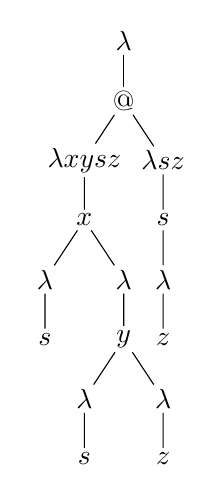
\begin{tikzpicture}[baseline=(root.base),level distance=5ex,inner ysep=0.5mm,sibling distance=10mm]
\node (root)
{$\lambda$}
child {node{$@$}
    child{node{$\lambda x y s z$}
        child { node{$x$}
            child{node{$\lambda$}{
                child {node {$s$}}}
            }
            child{node{$\lambda$}
                child{node{$y$}
                    child{node{$\lambda$}
                        child{ node {$s$}}
                    }
                    child{node{$\lambda$}
                        child{node{$z$}}}
                }
            }
        }
    }
    child{node{$\lambda s z$}
        child{node{$s$}
            child{node{$\lambda$} child{node{$z$}}}
        }
    }
}
;
\end{tikzpicture}

\begin{itemize}
\item Applying as many deterministic rules as possible gives the following traversal at which point the Opponent must make a choice:

$t_\epsilon = \Pstr[0.7cm]{(n0){\lambda }\ (n1){@}\ (n2-n1){\lambda x y s z}\ (n3-n2){x}\ (n4-n1){\lambda s z}\ (n5-n4){s}\ (n6-n3){\lambda }\ (n7-n2){s}\ (n8-n1){\ghostlmd^3}\ (n9-n0){\ghostvar^2} }$

(For readability we indicate the link label in exponent of the source node when representing traversals.)
The core of $t_\epsilon$ is
$t_\epsilon\filter\theroot = \Pstr[0.7cm]{(n0){\lambda } \cdot (n9-n0){{\ghostvar^2}} }$
and therefore $\pview{t_\epsilon\filter\theroot} =  \lambda \cdot \ghostvar^2$ is a path in  $\betanf{M}$.
This means that $\betanf{M}$ must be of the form $\lambda y s \ldots \cdot y N_1 \ldots \ldots N_q$ for some fresh variable $y$ and $s$ and $q\geq0$.

\item In order to determine what each argument $N_k$ is in the final normal form, we apply the $\rulename{IVar^\eta}$ rule for each possible argument index $k\geq 1$ and then continue applying the traversal rules.

For $k=1$ we get the traversal:

$t_1 = \Pstr[0.7cm]{(n0){\lambda }\ (n1){@}\ (n2-n1){\lambda x y s z}\ (n3-n2){x}\ (n4-n1){\lambda s z}\
(n5-n4){s}\ (n6-n3){\lambda }\
(n7-n2){s}\ (n8-n1){\ghostlmd^3}\
(n9-n0){\ghostvar^2}
(n10-n9){\ghostlmd^1}
(n11-n8){\ghostvar^1}
(n12-n7){\ghostlmd^1}
(n13-n6){\ghostvar^1}
(n14-n5){\lambda^1}
(n15-n4)z
(n16-n3){\lambda^2}
(n17-n2)y
(n18-n1){\ghostlmd^2}
(n19-n0){\ghostvar^1}
}$

The P-view of the traversal core is
$\pview{t_1\filter\theroot} = \Pstr[0.7cm]{(l){\lambda } \cdot (x-l){\ghostvar^2} \cdot (l1-x){\ghostlmd^1}
\cdot (x2-l){\ghostvar^1}
}$
which means that the normal form is of the form $\lambda y s \ldots \cdot s (y R_1 \ldots R_{q_2}) N_2 \ldots N_q$ for some terms $R_1$, \ldots $R_{q_2}$, and $q,q_2\geq 0$.

\item What should be the value of $q$? In other words, how many more $k$ do we need to look at?  The answer: we need to keep iterating on $k$ until the point where applying the traversal rules will only produce ghost variables and ghost lambda-nodes! Because there is a finite number of nodes in the computation tree, the variable node arities are bounded. Therefore for high enough argument indices $k$, the condition $i\leq|n|$     in the definition of \rulenamet{Var} will never be met:
        after applying rule \rulenamet{IVar^\eta} on $t_\epsilon$, all subsequent extensions of the traversal will be done using either rule $\rulename{Var^\eta}$ or rule $\rulename{Lam^\eta}$.
     The upper-bound $q$ for $k$ is precisely given by the \emph{arity threshold} of the traversal $t_\epsilon$ as defined in \ref{dfn:arity-threshold}.
     Here we have
     \begin{align*}
     \arth(t_\epsilon)
     = \max \{ & |s^2| , \\
               & |s^1| + (|s^2| - |\lambda|) , \\
               & |x| +  (|s^1| - |\lambda s z|) + (|s^2| - |\lambda|)
               %& |@| + (|x|- |\lambda x y s z |) + (|s^1| - |\lambda s z|) + (|s^2| -|\lambda|) \
               \} \\
    = \max \{   & 0 , \\
                & 1 + (0 - 0) , \\
                & 2 + (1 - 2) + (0 - 0)
                %& 2 + (2 - 4) + (1 - 2) + (0 - 0)
            \} \\
     = 1
     \end{align*}
     Thus we don't need to look at higher value of $k$ at $t_\epsilon$, we thus have:
     $\betanf{M} = \lambda y s \ldots \cdot s (y R_1 \ldots R_{q_2})$.

\item The arity threshold of $t_1$ is $\arth(t_1) = |z| + |y| - |\lambda^2| = 0+2-0 = 2$ hence  $\betanf{M}$ is of the form $\lambda y s \ldots \cdot s (y R_1 R_2)$.

\item Let's apply the rule \rulenamet{IVar^\eta} for varying value of child index $1\leq k_2 \leq q_2 = 2$. We first look at the case $k_2 = 1$. The traversal obtained is:

$t_{11} = \Pstr[0.7cm]{
(n0){\lambda }\
(n1){@}\ (n2-n1){\lambda x y s z}\ (n3-n2){x}\ (n4-n1){\lambda s z}\ (n5-n4){s}\ (n6-n3){\lambda }\ (n7-n2){s}\ (n8-n1){\ghostlmd^3}\ (n9-n0){\ghostvar^2}
(n10-n9){\ghostlmd^1}
(n11-n8){\ghostvar^1}
(n12-n7){\ghostlmd^1}
(n13-n6){\ghostvar^1}
(n14-n5){\lambda^1}
(n15-n4)z
(n16-n3){\lambda^2}
(n17-n2)y
(n18-n1){\ghostlmd^2}
(n19-n0){\ghostvar^1}
(n20-n19){\ghostlmd^1}
(n21-n18){\ghostvar^1}
(n22-n17,60:1)\lambda % points to non-ghost node
(n23-n2,45:3) s
(n24-n1,45:3) {\ghostlmd^3}
(n25-n0,48:2) {\ghostvar^2}
}$

Thus $\pview{t_{11} \filter\theroot} =
\Pstr[0.7cm]{
(n0){\lambda }\
 (n9-n0){\ghostvar^2}
 (n10-n9){\ghostlmd^1}
(n19-n0){\ghostvar^1}
(n20-n19){\ghostlmd^1}
(n25-n0,48:2){\ghostvar^2}
}$

Hence $\betanf{M}$ is of the form $\lambda y s \ldots \cdot s\ (y\ s\ R_2)$.

\item Now let's extend $t_1$ with \rulenamet{IVar^\lambda} for $k_2 = 2$. We get the traversal:

$t_{12} = \Pstr[0.7cm]{
(n0){\lambda }\
(n1){@}\ (n2-n1){\lambda x y s z}\
(n3-n2){x}\ (n4-n1){\lambda s z}\
(n5-n4){s}\
(n6-n3){\lambda }\
(n7-n2){s}\
(n8-n1){\ghostlmd^3}\
(n9-n0) {\ghostvar^2}
(n10-n9) {\ghostlmd^1}
(n11-n8){\ghostvar^1}
(n12-n7){\ghostlmd^1}
(n13-n6){\ghostvar^1}
(n14-n5)\lambda^1
(n15-n4)z
(n16-n3){\lambda^2}
(n17-n2)y
(n18-n1){\ghostlmd^2}
(n19-n0){\ghostvar^1}
(n20-n19){\ghostlmd^2} %%%%%%%%
(n21-n18){\ghostvar^2}
(n22-n17,60:2)\lambda % points to non-ghost node
(n23-n2,45:4) z
(n24-n1,45:4) {\ghostlmd^4}
(n25-n0,48:3) {\ghostvar^3}
}$

Thus $\pview{t_{12} \filter\theroot} =
\Pstr[0.7cm]{
(n0){\lambda }\
 (n9-n0){{\ghostvar^2}}
 (n10-n9){\ghostlmd^1}
(n19-n0){\ghostvar^1}
(n20-n19){\ghostlmd^2}
(n25-n0,48:3) {\ghostvar^3}
}$

Hence $\betanf{M} = \lambda y s z \cdot s\ (y\ s\ z)$.
\end{itemize}
\end{example}

\begin{example}[Baby example]
  Take $M = (\lambda x. x x) (\lambda y. y)$.

  $t = \Pstr[0.7cm]{(n0){\lambda }\ (n1){@}\ (n2-n1){\lambda x}\ (n3-n2){x}\ (n4-n1){\lambda y}\ (n5-n4){y}\ (n6-n3){\lambda }\ (n7-n2){x}\ (n8-n1){\lambda y}\ (n9-n8){y}\ (n10-n7){\ghostlmd^1}\ (n11-n6){\ghostvar^1}\ (n12-n5){\ghostlmd^{1}}\ (n13-n4){\ghostvar^2}\ (n14-n3){\ghostlmd^2}\ (n15-n2){\ghostvar^2}\ (n16-n1){\ghostlmd^2}\ (n17-n0){\ghostvar^1}}$

The traversal arity threshold is $arth(t) = 0$ therefore this the only maximal traversal. We have $\pview{t\filter\theroot} = \Pstr[0.7cm]{(n0){\lambda }\ (n17-n0){\ghostvar^1}}$ thus the beta-normal form of $M$ is $\lambda y . y$.
\end{example}

\begin{example}[Neil Jones' $varity\ 2$]

Take $M = varity\ two$ where
\begin{align*}
  varity &\equiv \lambda t.t (\lambda n a x . n (\lambda s z . a s (x s z))) (\lambda a. a) (\lambda z_0 . z_0) \\
  two &\equiv \lambda s_2 z_2 . s_2 (s_2\ z_2)
\end{align*}

In order to compute the set of normalizing traversals, we apply the traversal rules inductively until an input variable is reached, at which point we apply the rule \rulenamet{IVar^\eta} for all possible values of $k$ ranging from $1$ to the arity threshold of the traversal. The first traversal obtained is denoted $t_\epsilon$, and for every sequence of integer $s \in \nat^*$,  the traversal $t_{s \cdot k}$ represents the maximal traversal obtained after extending $t_s$ using the rule \rulenamet{IVar^\eta} with link-label $k \in \nat$.
This process yields the set of traversals $\{t_\epsilon, t_{11}, t_{12}, t_{121}, t_{122} \}$ represented in the following pages.

\begin{landscape}
\resizebox{1.1\hsize}{!}{$
t_\epsilon = \Pstr[0.7cm]{(n0){\lambda }\ (n1){@}\ (n2-n1){\lambda t}\ (n3-n2){t}\ (n4-n1){\lambda s_2 z_2}\ (n5-n4){s_2}\ (n6-n3){\lambda n a x}\ (n7-n6){n}\ (n8-n5){\lambda }\ (n9-n4){s_2}\ (n10-n3){\lambda n a x}\ (n11-n10){n}\ (n12-n9){\lambda }\ (n13-n4){z_2}\ (n14-n3){\lambda a}\ (n15-n14){a}\ (n16-n13){{\ghostlmd^{1}}}\ (n17-n12){{\ghostvar^{1}}}\ (n18-n11){\lambda s z}\ (n19-n10){a}\ (n20-n9){{\ghostlmd^{2}}}\ (n21-n8){{\ghostvar^{1}}}\ (n22-n7){\lambda s z}\ (n23-n6){a}\ (n24-n5){{\ghostlmd^{2}}}\ (n25-n4){{\ghostvar^{3}}}\
(n26-n3){\lambda z0}\ (n27-n26){z0}\ (n28-n25){{\ghostlmd^{1}}}\ (n29-n24){{\ghostvar^{1}}}\
(n30-n23){\lambda }\ (n31-n22){s}\ (n32-n21){{\ghostlmd^{1}}}\ (n33-n20){{\ghostvar^{1}}}\ (n34-n19){\lambda }\ (n35-n18){s}\ (n36-n17){{\ghostlmd^{1}}}\ (n37-n16){{\ghostvar^{1}}}\ (n38-n15){{\ghostlmd^{1}}}\ (n39-n14){{\ghostvar^{2}}}\ (n40-n13){{\ghostlmd^{2}}}\ (n41-n12){{\ghostvar^{2}}}\ (n42-n11){{\ghostlmd^{2}}}\ (n43-n10){{\ghostvar^{4}}}\ (n44-n9){{\ghostlmd^{4}}}\ (n45-n8){{\ghostvar^{3}}}\ (n46-n7){{\ghostlmd^{3}}}\ (n47-n6){{\ghostvar^{5}}}\ (n48-n5){{\ghostlmd^{5}}}\ (n49-n4){{\ghostvar^{6}}}\ (n50-n3){{\ghostlmd^{6}}}\ (n51-n2){{\ghostvar^{4}}}\ (n52-n1){{\ghostlmd^{4}}}\ (n53-n0){{\ghostvar^{3}}}}$}

\resizebox{1.1\hsize}{!}{$t_{1} = \Pstr[0.7cm]{(n0){\lambda }\ (n1){@}\ (n2-n1){\lambda t}\ (n3-n2){t}\ (n4-n1){\lambda s_2 z_2}\ (n5-n4){s_2}\ (n6-n3){\lambda n a x}\ (n7-n6){n}\ (n8-n5){\lambda }\ (n9-n4){s_2}\ (n10-n3){\lambda n a x}\ (n11-n10){n}\ (n12-n9){\lambda }\ (n13-n4){z_2}\ (n14-n3){\lambda a}\ (n15-n14){a}\ (n16-n13){{\ghostlmd^{1}}}\ (n17-n12){{\ghostvar^{1}}}\ (n18-n11){\lambda s z}\ (n19-n10){a}\ (n20-n9){{\ghostlmd^{2}}}\ (n21-n8){{\ghostvar^{1}}}\ (n22-n7){\lambda s z}\ (n23-n6){a}\ (n24-n5){{\ghostlmd^{2}}}\ (n25-n4){{\ghostvar^{3}}}\ (n26-n3){\lambda z0}\ (n27-n26){z0}\ (n28-n25){{\ghostlmd^{1}}}\ (n29-n24){{\ghostvar^{1}}}\ (n30-n23){\lambda }\ (n31-n22){s}\ (n32-n21){{\ghostlmd^{1}}}\ (n33-n20){{\ghostvar^{1}}}\ (n34-n19){\lambda }\ (n35-n18){s}\ (n36-n17){{\ghostlmd^{1}}}\ (n37-n16){{\ghostvar^{1}}}\ (n38-n15){{\ghostlmd^{1}}}\ (n39-n14){{\ghostvar^{2}}}\ (n40-n13){{\ghostlmd^{2}}}\ (n41-n12){{\ghostvar^{2}}}\ (n42-n11){{\ghostlmd^{2}}}\ (n43-n10){{\ghostvar^{4}}}\ (n44-n9){{\ghostlmd^{4}}}\ (n45-n8){{\ghostvar^{3}}}\ (n46-n7){{\ghostlmd^{3}}}\ (n47-n6){{\ghostvar^{5}}}\ (n48-n5){{\ghostlmd^{5}}}\ (n49-n4){{\ghostvar^{6}}}\ (n50-n3){{\ghostlmd^{6}}}\ (n51-n2){{\ghostvar^{4}}}\ (n52-n1){{\ghostlmd^{4}}}\ (n53-n0){{\ghostvar^{3}}}\ (n54-n53){{\ghostlmd^{1}}}\ (n55-n52){{\ghostvar^{1}}}\ (n56-n51){{\ghostlmd^{1}}}\ (n57-n50){{\ghostvar^{1}}}\ (n58-n49){{\ghostlmd^{1}}}\ (n59-n48){{\ghostvar^{1}}}\ (n60-n47){{\ghostlmd^{1}}}\ (n61-n46){{\ghostvar^{1}}}\ (n62-n45){{\ghostlmd^{1}}}\ (n63-n44){{\ghostvar^{1}}}\ (n64-n43){{\ghostlmd^{1}}}\ (n65-n42){{\ghostvar^{1}}}\ (n66-n41){{\ghostlmd^{1}}}\ (n67-n40){{\ghostvar^{1}}}\ (n68-n39){{\ghostlmd^{1}}}\ (n69-n38){{\ghostvar^{1}}}\ (n70-n37){{\ghostlmd^{1}}}\ (n71-n36){{\ghostvar^{1}}}\ (n72-n35){{\ghostlmd^{1}}}\ (n73-n34){{\ghostvar^{1}}}\ (n74-n33){{\ghostlmd^{1}}}\ (n75-n32){{\ghostvar^{1}}}\ (n76-n31){{\ghostlmd^{1}}}\ (n77-n30){{\ghostvar^{1}}}\ (n78-n29){{\ghostlmd^{1}}}\ (n79-n28){{\ghostvar^{1}}}\ (n80-n27){{\ghostlmd^{1}}}\ (n81-n26){{\ghostvar^{2}}}\ (n82-n25){{\ghostlmd^{2}}}\ (n83-n24){{\ghostvar^{2}}}\ (n84-n23){\lambda }\ (n85-n6){x}\ (n86-n5){{\ghostlmd^{3}}}\ (n87-n4){{\ghostvar^{4}}}\ (n88-n3){{\ghostlmd^{4}}}\ (n89-n2){{\ghostvar^{2}}}\ (n90-n1){{\ghostlmd^{2}}}\ (n91-n0){{\ghostvar^{1}}}}$}


\resizebox{1.1\hsize}{!}{$t_{11} = \Pstr[0.7cm]{(n0){\lambda }\ (n1){@}\ (n2-n1){\lambda t}\ (n3-n2){t}\ (n4-n1){\lambda s_2 z_2}\ (n5-n4){s_2}\ (n6-n3){\lambda n a x}\ (n7-n6){n}\ (n8-n5){\lambda }\ (n9-n4){s_2}\ (n10-n3){\lambda n a x}\ (n11-n10){n}\ (n12-n9){\lambda }\ (n13-n4){z_2}\ (n14-n3){\lambda a}\ (n15-n14){a}\ (n16-n13){{\ghostlmd^{1}}}\ (n17-n12){{\ghostvar^{1}}}\ (n18-n11){\lambda s z}\ (n19-n10){a}\ (n20-n9){{\ghostlmd^{2}}}\ (n21-n8){{\ghostvar^{1}}}\ (n22-n7){\lambda s z}\ (n23-n6){a}\ (n24-n5){{\ghostlmd^{2}}}\ (n25-n4){{\ghostvar^{3}}}\ (n26-n3){\lambda z0}\ (n27-n26){z0}\ (n28-n25){{\ghostlmd^{1}}}\ (n29-n24){{\ghostvar^{1}}}\ (n30-n23){\lambda }\ (n31-n22){s}\ (n32-n21){{\ghostlmd^{1}}}\ (n33-n20){{\ghostvar^{1}}}\ (n34-n19){\lambda }\ (n35-n18){s}\ (n36-n17){{\ghostlmd^{1}}}\ (n37-n16){{\ghostvar^{1}}}\ (n38-n15){{\ghostlmd^{1}}}\ (n39-n14){{\ghostvar^{2}}}\ (n40-n13){{\ghostlmd^{2}}}\ (n41-n12){{\ghostvar^{2}}}\ (n42-n11){{\ghostlmd^{2}}}\ (n43-n10){{\ghostvar^{4}}}\ (n44-n9){{\ghostlmd^{4}}}\ (n45-n8){{\ghostvar^{3}}}\ (n46-n7){{\ghostlmd^{3}}}\ (n47-n6){{\ghostvar^{5}}}\ (n48-n5){{\ghostlmd^{5}}}\ (n49-n4){{\ghostvar^{6}}}\ (n50-n3){{\ghostlmd^{6}}}\ (n51-n2){{\ghostvar^{4}}}\ (n52-n1){{\ghostlmd^{4}}}\ (n53-n0){{\ghostvar^{3}}}\ (n54-n53){{\ghostlmd^{1}}}\ (n55-n52){{\ghostvar^{1}}}\ (n56-n51){{\ghostlmd^{1}}}\ (n57-n50){{\ghostvar^{1}}}\ (n58-n49){{\ghostlmd^{1}}}\ (n59-n48){{\ghostvar^{1}}}\ (n60-n47){{\ghostlmd^{1}}}\ (n61-n46){{\ghostvar^{1}}}\ (n62-n45){{\ghostlmd^{1}}}\ (n63-n44){{\ghostvar^{1}}}\ (n64-n43){{\ghostlmd^{1}}}\ (n65-n42){{\ghostvar^{1}}}\ (n66-n41){{\ghostlmd^{1}}}\ (n67-n40){{\ghostvar^{1}}}\ (n68-n39){{\ghostlmd^{1}}}\ (n69-n38){{\ghostvar^{1}}}\ (n70-n37){{\ghostlmd^{1}}}\ (n71-n36){{\ghostvar^{1}}}\ (n72-n35){{\ghostlmd^{1}}}\ (n73-n34){{\ghostvar^{1}}}\ (n74-n33){{\ghostlmd^{1}}}\ (n75-n32){{\ghostvar^{1}}}\ (n76-n31){{\ghostlmd^{1}}}\ (n77-n30){{\ghostvar^{1}}}\ (n78-n29){{\ghostlmd^{1}}}\ (n79-n28){{\ghostvar^{1}}}\ (n80-n27){{\ghostlmd^{1}}}\ (n81-n26){{\ghostvar^{2}}}\ (n82-n25){{\ghostlmd^{2}}}\ (n83-n24){{\ghostvar^{2}}}\ (n84-n23){\lambda }\ (n85-n6){x}\ (n86-n5){{\ghostlmd^{3}}}\ (n87-n4){{\ghostvar^{4}}}\ (n88-n3){{\ghostlmd^{4}}}\ (n89-n2){{\ghostvar^{2}}}\ (n90-n1){{\ghostlmd^{2}}}\ (n91-n0){{\ghostvar^{1}}}\ (n92-n91){{\ghostlmd^{1}}}\ (n93-n90){{\ghostvar^{1}}}\ (n94-n89){{\ghostlmd^{1}}}\ (n95-n88){{\ghostvar^{1}}}\ (n96-n87){{\ghostlmd^{1}}}\ (n97-n86){{\ghostvar^{1}}}\ (n98-n85){\lambda }\ (n99-n22){s}\ (n100-n21){{\ghostlmd^{1}}}\ (n101-n20){{\ghostvar^{1}}}\ (n102-n19){\lambda }\ (n103-n18){s}\ (n104-n17){{\ghostlmd^{1}}}\ (n105-n16){{\ghostvar^{1}}}\ (n106-n15){{\ghostlmd^{1}}}\ (n107-n14){{\ghostvar^{2}}}\ (n108-n13){{\ghostlmd^{2}}}\ (n109-n12){{\ghostvar^{2}}}\ (n110-n11){{\ghostlmd^{2}}}\ (n111-n10){{\ghostvar^{4}}}\ (n112-n9){{\ghostlmd^{4}}}\ (n113-n8){{\ghostvar^{3}}}\ (n114-n7){{\ghostlmd^{3}}}\ (n115-n6){{\ghostvar^{5}}}\ (n116-n5){{\ghostlmd^{5}}}\ (n117-n4){{\ghostvar^{6}}}\ (n118-n3){{\ghostlmd^{6}}}\ (n119-n2){{\ghostvar^{4}}}\ (n120-n1){{\ghostlmd^{4}}}\ (n121-n0){{\ghostvar^{3}}}}$}

\resizebox{1.1\hsize}{!}{$t_{12} = \Pstr[0.7cm]{(n0){\lambda }\ (n1){@}\ (n2-n1){\lambda t}\ (n3-n2){t}\ (n4-n1){\lambda s_2 z_2}\ (n5-n4){s_2}\ (n6-n3){\lambda n a x}\ (n7-n6){n}\ (n8-n5){\lambda }\ (n9-n4){s_2}\ (n10-n3){\lambda n a x}\ (n11-n10){n}\ (n12-n9){\lambda }\ (n13-n4){z_2}\ (n14-n3){\lambda a}\ (n15-n14){a}\ (n16-n13){{\ghostlmd^{1}}}\ (n17-n12){{\ghostvar^{1}}}\ (n18-n11){\lambda s z}\ (n19-n10){a}\ (n20-n9){{\ghostlmd^{2}}}\ (n21-n8){{\ghostvar^{1}}}\ (n22-n7){\lambda s z}\ (n23-n6){a}\ (n24-n5){{\ghostlmd^{2}}}\ (n25-n4){{\ghostvar^{3}}}\ (n26-n3){\lambda z0}\ (n27-n26){z0}\ (n28-n25){{\ghostlmd^{1}}}\ (n29-n24){{\ghostvar^{1}}}\ (n30-n23){\lambda }\ (n31-n22){s}\ (n32-n21){{\ghostlmd^{1}}}\ (n33-n20){{\ghostvar^{1}}}\ (n34-n19){\lambda }\ (n35-n18){s}\ (n36-n17){{\ghostlmd^{1}}}\ (n37-n16){{\ghostvar^{1}}}\ (n38-n15){{\ghostlmd^{1}}}\ (n39-n14){{\ghostvar^{2}}}\ (n40-n13){{\ghostlmd^{2}}}\ (n41-n12){{\ghostvar^{2}}}\ (n42-n11){{\ghostlmd^{2}}}\ (n43-n10){{\ghostvar^{4}}}\ (n44-n9){{\ghostlmd^{4}}}\ (n45-n8){{\ghostvar^{3}}}\ (n46-n7){{\ghostlmd^{3}}}\ (n47-n6){{\ghostvar^{5}}}\ (n48-n5){{\ghostlmd^{5}}}\ (n49-n4){{\ghostvar^{6}}}\ (n50-n3){{\ghostlmd^{6}}}\ (n51-n2){{\ghostvar^{4}}}\ (n52-n1){{\ghostlmd^{4}}}\ (n53-n0){{\ghostvar^{3}}}\ (n54-n53){{\ghostlmd^{1}}}\ (n55-n52){{\ghostvar^{1}}}\ (n56-n51){{\ghostlmd^{1}}}\ (n57-n50){{\ghostvar^{1}}}\ (n58-n49){{\ghostlmd^{1}}}\ (n59-n48){{\ghostvar^{1}}}\ (n60-n47){{\ghostlmd^{1}}}\ (n61-n46){{\ghostvar^{1}}}\ (n62-n45){{\ghostlmd^{1}}}\ (n63-n44){{\ghostvar^{1}}}\ (n64-n43){{\ghostlmd^{1}}}\ (n65-n42){{\ghostvar^{1}}}\ (n66-n41){{\ghostlmd^{1}}}\ (n67-n40){{\ghostvar^{1}}}\ (n68-n39){{\ghostlmd^{1}}}\ (n69-n38){{\ghostvar^{1}}}\ (n70-n37){{\ghostlmd^{1}}}\ (n71-n36){{\ghostvar^{1}}}\ (n72-n35){{\ghostlmd^{1}}}\ (n73-n34){{\ghostvar^{1}}}\ (n74-n33){{\ghostlmd^{1}}}\ (n75-n32){{\ghostvar^{1}}}\ (n76-n31){{\ghostlmd^{1}}}\ (n77-n30){{\ghostvar^{1}}}\ (n78-n29){{\ghostlmd^{1}}}\ (n79-n28){{\ghostvar^{1}}}\ (n80-n27){{\ghostlmd^{1}}}\ (n81-n26){{\ghostvar^{2}}}\ (n82-n25){{\ghostlmd^{2}}}\ (n83-n24){{\ghostvar^{2}}}\ (n84-n23){\lambda }\ (n85-n6){x}\ (n86-n5){{\ghostlmd^{3}}}\ (n87-n4){{\ghostvar^{4}}}\ (n88-n3){{\ghostlmd^{4}}}\ (n89-n2){{\ghostvar^{2}}}\ (n90-n1){{\ghostlmd^{2}}}\ (n91-n0){{\ghostvar^{1}}}\ (n92-n91){{\ghostlmd^{2}}}\ (n93-n90){{\ghostvar^{2}}}\ (n94-n89){{\ghostlmd^{2}}}\ (n95-n88){{\ghostvar^{2}}}\ (n96-n87){{\ghostlmd^{2}}}\ (n97-n86){{\ghostvar^{2}}}\ (n98-n85){\lambda }\ (n99-n22){z}\ (n100-n21){{\ghostlmd^{2}}}\ (n101-n20){{\ghostvar^{2}}}\ (n102-n19){\lambda }\ (n103-n10){x}\ (n104-n9){{\ghostlmd^{3}}}\ (n105-n8){{\ghostvar^{2}}}\ (n106-n7){{\ghostlmd^{2}}}\ (n107-n6){{\ghostvar^{4}}}\ (n108-n5){{\ghostlmd^{4}}}\ (n109-n4){{\ghostvar^{5}}}\ (n110-n3){{\ghostlmd^{5}}}\ (n111-n2){{\ghostvar^{3}}}\ (n112-n1){{\ghostlmd^{3}}}\ (n113-n0){{\ghostvar^{2}}}}$}


\resizebox{1.1\hsize}{!}{$t_{121} =
\Pstr[0.7cm]{(n0){\lambda }\ (n1){@}\ (n2-n1){\lambda t}\ (n3-n2){t}\ (n4-n1){\lambda s_2 z_2}\ (n5-n4){s_2}\ (n6-n3){\lambda n a x}\ (n7-n6){n}\ (n8-n5){\lambda }\ (n9-n4){s_2}\ (n10-n3){\lambda n a x}\ (n11-n10){n}\ (n12-n9){\lambda }\ (n13-n4){z_2}\ (n14-n3){\lambda a}\ (n15-n14){a}\ (n16-n13){{\ghostlmd^{1}}}\ (n17-n12){{\ghostvar^{1}}}\ (n18-n11){\lambda s z}\ (n19-n10){a}\ (n20-n9){{\ghostlmd^{2}}}\ (n21-n8){{\ghostvar^{1}}}\ (n22-n7){\lambda s z}\ (n23-n6){a}\ (n24-n5){{\ghostlmd^{2}}}\ (n25-n4){{\ghostvar^{3}}}\ (n26-n3){\lambda z0}\ (n27-n26){z0}\ (n28-n25){{\ghostlmd^{1}}}\ (n29-n24){{\ghostvar^{1}}}\ (n30-n23){\lambda }\ (n31-n22){s}\ (n32-n21){{\ghostlmd^{1}}}\ (n33-n20){{\ghostvar^{1}}}\ (n34-n19){\lambda }\ (n35-n18){s}\ (n36-n17){{\ghostlmd^{1}}}\ (n37-n16){{\ghostvar^{1}}}\ (n38-n15){{\ghostlmd^{1}}}\ (n39-n14){{\ghostvar^{2}}}\ (n40-n13){{\ghostlmd^{2}}}\ (n41-n12){{\ghostvar^{2}}}\ (n42-n11){{\ghostlmd^{2}}}\ (n43-n10){{\ghostvar^{4}}}\ (n44-n9){{\ghostlmd^{4}}}\ (n45-n8){{\ghostvar^{3}}}\ (n46-n7){{\ghostlmd^{3}}}\ (n47-n6){{\ghostvar^{5}}}\ (n48-n5){{\ghostlmd^{5}}}\ (n49-n4){{\ghostvar^{6}}}\ (n50-n3){{\ghostlmd^{6}}}\ (n51-n2){{\ghostvar^{4}}}\ (n52-n1){{\ghostlmd^{4}}}\ (n53-n0){{\ghostvar^{3}}}\ (n54-n53){{\ghostlmd^{1}}}\ (n55-n52){{\ghostvar^{1}}}\ (n56-n51){{\ghostlmd^{1}}}\ (n57-n50){{\ghostvar^{1}}}\ (n58-n49){{\ghostlmd^{1}}}\ (n59-n48){{\ghostvar^{1}}}\ (n60-n47){{\ghostlmd^{1}}}\ (n61-n46){{\ghostvar^{1}}}\ (n62-n45){{\ghostlmd^{1}}}\ (n63-n44){{\ghostvar^{1}}}\ (n64-n43){{\ghostlmd^{1}}}\ (n65-n42){{\ghostvar^{1}}}\ (n66-n41){{\ghostlmd^{1}}}\ (n67-n40){{\ghostvar^{1}}}\ (n68-n39){{\ghostlmd^{1}}}\ (n69-n38){{\ghostvar^{1}}}\ (n70-n37){{\ghostlmd^{1}}}\ (n71-n36){{\ghostvar^{1}}}\ (n72-n35){{\ghostlmd^{1}}}\ (n73-n34){{\ghostvar^{1}}}\ (n74-n33){{\ghostlmd^{1}}}\ (n75-n32){{\ghostvar^{1}}}\ (n76-n31){{\ghostlmd^{1}}}\ (n77-n30){{\ghostvar^{1}}}\ (n78-n29){{\ghostlmd^{1}}}\ (n79-n28){{\ghostvar^{1}}}\ (n80-n27){{\ghostlmd^{1}}}\ (n81-n26){{\ghostvar^{2}}}\ (n82-n25){{\ghostlmd^{2}}}\ (n83-n24){{\ghostvar^{2}}}\ (n84-n23){\lambda }\ (n85-n6){x}\ (n86-n5){{\ghostlmd^{3}}}\ (n87-n4){{\ghostvar^{4}}}\ (n88-n3){{\ghostlmd^{4}}}\ (n89-n2){{\ghostvar^{2}}}\ (n90-n1){{\ghostlmd^{2}}}\ (n91-n0){{\ghostvar^{1}}}\ (n92-n91){{\ghostlmd^{2}}}\ (n93-n90){{\ghostvar^{2}}}\ (n94-n89){{\ghostlmd^{2}}}\ (n95-n88){{\ghostvar^{2}}}\ (n96-n87){{\ghostlmd^{2}}}\ (n97-n86){{\ghostvar^{2}}}\ (n98-n85){\lambda }\ (n99-n22){z}\ (n100-n21){{\ghostlmd^{2}}}\ (n101-n20){{\ghostvar^{2}}}\ (n102-n19){\lambda }\ (n103-n10){x}\ (n104-n9){{\ghostlmd^{3}}}\ (n105-n8){{\ghostvar^{2}}}\ (n106-n7){{\ghostlmd^{2}}}\ (n107-n6){{\ghostvar^{4}}}\ (n108-n5){{\ghostlmd^{4}}}\ (n109-n4){{\ghostvar^{5}}}\ (n110-n3){{\ghostlmd^{5}}}\ (n111-n2){{\ghostvar^{3}}}\ (n112-n1){{\ghostlmd^{3}}}\ (n113-n0){{\ghostvar^{2}}}\ (n114-n113){{\ghostlmd^{1}}}\ (n115-n112){{\ghostvar^{1}}}\ (n116-n111){{\ghostlmd^{1}}}\ (n117-n110){{\ghostvar^{1}}}\ (n118-n109){{\ghostlmd^{1}}}\ (n119-n108){{\ghostvar^{1}}}\ (n120-n107){{\ghostlmd^{1}}}\ (n121-n106){{\ghostvar^{1}}}\ (n122-n105){{\ghostlmd^{1}}}\ (n123-n104){{\ghostvar^{1}}}\ (n124-n103){\lambda }\ (n125-n18){s}\ (n126-n17){{\ghostlmd^{1}}}\ (n127-n16){{\ghostvar^{1}}}\ (n128-n15){{\ghostlmd^{1}}}\ (n129-n14){{\ghostvar^{2}}}\ (n130-n13){{\ghostlmd^{2}}}\ (n131-n12){{\ghostvar^{2}}}\ (n132-n11){{\ghostlmd^{2}}}\ (n133-n10){{\ghostvar^{4}}}\ (n134-n9){{\ghostlmd^{4}}}\ (n135-n8){{\ghostvar^{3}}}\ (n136-n7){{\ghostlmd^{3}}}\ (n137-n6){{\ghostvar^{5}}}\ (n138-n5){{\ghostlmd^{5}}}\ (n139-n4){{\ghostvar^{6}}}\ (n140-n3){{\ghostlmd^{6}}}\ (n141-n2){{\ghostvar^{4}}}\ (n142-n1){{\ghostlmd^{4}}}\ (n143-n0){{\ghostvar^{3}}}}$}

\resizebox{1.1\hsize}{!}{$t_{122} =
\Pstr[0.7cm]{(n0){\lambda }\ (n1){@}\ (n2-n1){\lambda t}\ (n3-n2){t}\ (n4-n1){\lambda s_2 z_2}\ (n5-n4){s_2}\ (n6-n3){\lambda n a x}\ (n7-n6){n}\ (n8-n5){\lambda }\ (n9-n4){s_2}\ (n10-n3){\lambda n a x}\ (n11-n10){n}\ (n12-n9){\lambda }\ (n13-n4){z_2}\ (n14-n3){\lambda a}\ (n15-n14){a}\ (n16-n13){{\ghostlmd^{1}}}\ (n17-n12){{\ghostvar^{1}}}\ (n18-n11){\lambda s z}\ (n19-n10){a}\ (n20-n9){{\ghostlmd^{2}}}\ (n21-n8){{\ghostvar^{1}}}\ (n22-n7){\lambda s z}\ (n23-n6){a}\ (n24-n5){{\ghostlmd^{2}}}\ (n25-n4){{\ghostvar^{3}}}\ (n26-n3){\lambda z0}\ (n27-n26){z0}\ (n28-n25){{\ghostlmd^{1}}}\ (n29-n24){{\ghostvar^{1}}}\ (n30-n23){\lambda }\ (n31-n22){s}\ (n32-n21){{\ghostlmd^{1}}}\ (n33-n20){{\ghostvar^{1}}}\ (n34-n19){\lambda }\ (n35-n18){s}\ (n36-n17){{\ghostlmd^{1}}}\ (n37-n16){{\ghostvar^{1}}}\ (n38-n15){{\ghostlmd^{1}}}\ (n39-n14){{\ghostvar^{2}}}\ (n40-n13){{\ghostlmd^{2}}}\ (n41-n12){{\ghostvar^{2}}}\ (n42-n11){{\ghostlmd^{2}}}\ (n43-n10){{\ghostvar^{4}}}\ (n44-n9){{\ghostlmd^{4}}}\ (n45-n8){{\ghostvar^{3}}}\ (n46-n7){{\ghostlmd^{3}}}\ (n47-n6){{\ghostvar^{5}}}\ (n48-n5){{\ghostlmd^{5}}}\ (n49-n4){{\ghostvar^{6}}}\ (n50-n3){{\ghostlmd^{6}}}\ (n51-n2){{\ghostvar^{4}}}\ (n52-n1){{\ghostlmd^{4}}}\ (n53-n0){{\ghostvar^{3}}}\ (n54-n53){{\ghostlmd^{1}}}\ (n55-n52){{\ghostvar^{1}}}\ (n56-n51){{\ghostlmd^{1}}}\ (n57-n50){{\ghostvar^{1}}}\ (n58-n49){{\ghostlmd^{1}}}\ (n59-n48){{\ghostvar^{1}}}\ (n60-n47){{\ghostlmd^{1}}}\ (n61-n46){{\ghostvar^{1}}}\ (n62-n45){{\ghostlmd^{1}}}\ (n63-n44){{\ghostvar^{1}}}\ (n64-n43){{\ghostlmd^{1}}}\ (n65-n42){{\ghostvar^{1}}}\ (n66-n41){{\ghostlmd^{1}}}\ (n67-n40){{\ghostvar^{1}}}\ (n68-n39){{\ghostlmd^{1}}}\ (n69-n38){{\ghostvar^{1}}}\ (n70-n37){{\ghostlmd^{1}}}\ (n71-n36){{\ghostvar^{1}}}\ (n72-n35){{\ghostlmd^{1}}}\ (n73-n34){{\ghostvar^{1}}}\ (n74-n33){{\ghostlmd^{1}}}\ (n75-n32){{\ghostvar^{1}}}\ (n76-n31){{\ghostlmd^{1}}}\ (n77-n30){{\ghostvar^{1}}}\ (n78-n29){{\ghostlmd^{1}}}\ (n79-n28){{\ghostvar^{1}}}\ (n80-n27){{\ghostlmd^{1}}}\ (n81-n26){{\ghostvar^{2}}}\ (n82-n25){{\ghostlmd^{2}}}\ (n83-n24){{\ghostvar^{2}}}\ (n84-n23){\lambda }\ (n85-n6){x}\ (n86-n5){{\ghostlmd^{3}}}\ (n87-n4){{\ghostvar^{4}}}\ (n88-n3){{\ghostlmd^{4}}}\ (n89-n2){{\ghostvar^{2}}}\ (n90-n1){{\ghostlmd^{2}}}\ (n91-n0){{\ghostvar^{1}}}\ (n92-n91){{\ghostlmd^{2}}}\ (n93-n90){{\ghostvar^{2}}}\ (n94-n89){{\ghostlmd^{2}}}\ (n95-n88){{\ghostvar^{2}}}\ (n96-n87){{\ghostlmd^{2}}}\ (n97-n86){{\ghostvar^{2}}}\ (n98-n85){\lambda }\ (n99-n22){z}\ (n100-n21){{\ghostlmd^{2}}}\ (n101-n20){{\ghostvar^{2}}}\ (n102-n19){\lambda }\ (n103-n10){x}\ (n104-n9){{\ghostlmd^{3}}}\ (n105-n8){{\ghostvar^{2}}}\ (n106-n7){{\ghostlmd^{2}}}\ (n107-n6){{\ghostvar^{4}}}\ (n108-n5){{\ghostlmd^{4}}}\ (n109-n4){{\ghostvar^{5}}}\ (n110-n3){{\ghostlmd^{5}}}\ (n111-n2){{\ghostvar^{3}}}\ (n112-n1){{\ghostlmd^{3}}}\ (n113-n0){{\ghostvar^{2}}}\ (n114-n113){{\ghostlmd^{2}}}\ (n115-n112){{\ghostvar^{2}}}\ (n116-n111){{\ghostlmd^{2}}}\ (n117-n110){{\ghostvar^{2}}}\ (n118-n109){{\ghostlmd^{2}}}\ (n119-n108){{\ghostvar^{2}}}\ (n120-n107){{\ghostlmd^{2}}}\ (n121-n106){{\ghostvar^{2}}}\ (n122-n105){{\ghostlmd^{2}}}\ (n123-n104){{\ghostvar^{2}}}\ (n124-n103){\lambda }\ (n125-n18){z}\ (n126-n17){{\ghostlmd^{2}}}\ (n127-n16){{\ghostvar^{2}}}\ (n128-n15){{\ghostlmd^{2}}}\ (n129-n14){{\ghostvar^{3}}}\ (n130-n13){{\ghostlmd^{3}}}\ (n131-n12){{\ghostvar^{3}}}\ (n132-n11){{\ghostlmd^{3}}}\ (n133-n10){{\ghostvar^{5}}}\ (n134-n9){{\ghostlmd^{5}}}\ (n135-n8){{\ghostvar^{4}}}\ (n136-n7){{\ghostlmd^{4}}}\ (n137-n6){{\ghostvar^{6}}}\ (n138-n5){{\ghostlmd^{6}}}\ (n139-n4){{\ghostvar^{7}}}\ (n140-n3){{\ghostlmd^{7}}}\ (n141-n2){{\ghostvar^{5}}}\ (n142-n1){{\ghostlmd^{5}}}\ (n143-n0){{\ghostvar^{4}}}}$}
\end{landscape}

Keeping only the maximal traversals gives us the set of normalizing traversals of $M$:
$$\travset^s(M) = \{ t_{11}, t_{121}, t_{122} \}$$

Hence the set of maximal paths in the beta-normal form of $M$ is given by:
\begin{align*}
\pview{t_{11} \filter \theroot} &=
    \Pstr[0.7cm]{(n0){\lambda }\ (n1-n0){{\ghostvar^{3}}}\ (n2-n1){{\ghostlmd^{1}}}\ (n3-n0){{\ghostvar^{1}}}\ (n4-n3){{\ghostlmd^{1}}}\ (n5-n0){{\ghostvar^{3}}}}
\\
\pview{t_{121} \filter \theroot} &=
    \Pstr[0.7cm]{(n0){\lambda }\ (n1-n0){{\ghostvar^{3}}}\ (n2-n1){{\ghostlmd^{1}}}\ (n3-n0){{\ghostvar^{1}}}\ (n4-n3){{\ghostlmd^{2}}}\ (n5-n0){{\ghostvar^{2}}}\ (n6-n5){{\ghostlmd^{1}}}\ (n7-n0){{\ghostvar^{3}}}}
\\
\pview{t_{122} \filter \theroot} &=
\Pstr[0.7cm]{(n0){\lambda }\ (n1-n0){{\ghostvar^{3}}}\ (n2-n1){{\ghostlmd^{1}}}\ (n3-n0){{\ghostvar^{1}}}\ (n4-n3){{\ghostlmd^{2}}}\ (n5-n0){{\ghostvar^{2}}}\ (n6-n5){{\ghostlmd^{2}}}\ (n7-n0){{\ghostvar^{4}}}}
\end{align*}

Therefore the beta-normal from of $arity\ two$ is:
\begin{align*}
\betanf{varity\ two} &= \lambda x_1 x_2 x_3 x_4 . x_3 (x_1 x_3 (x_2 x_3 x_4))\\
&\equiv_\alpha \lambda x y s z . s (x s (y s z))
\end{align*}



\end{example}
\bibliographystyle{abbrv}
\bibliography{ulctrav}

\end{document}
